\section{Практические задания}
\subsection*{Постановка задачи}
     Студентам предлагается написать программу, имитирующую преобразования и процессы, происходящие с сигналом в рамках OFDM- модуляции, на всех трех этапах его существования: образования, передачи и приема.
     Выполнять задание можно на любом удобном языке программирования (приоритетные языки matlab, python). 
     Данная глава содержит последовательное описание каждого этапа и ожидаемые промежуточные результаты.
    
Разработка модели состоит из пяти этапов, на каждом из которых сигнал проходит полный 'жизненный цикл', то есть кодирование бит, формирование сигнала, передачу в канал, прием и декодирование.  
На каждом этапе нам предстоит добавлять новые элементы обработки сигнала, учитывающие реальные физические процессы. Полная схема модели приведена на Рис.\ref{fg:schem0} 

\begin{figure}[H]
\centering
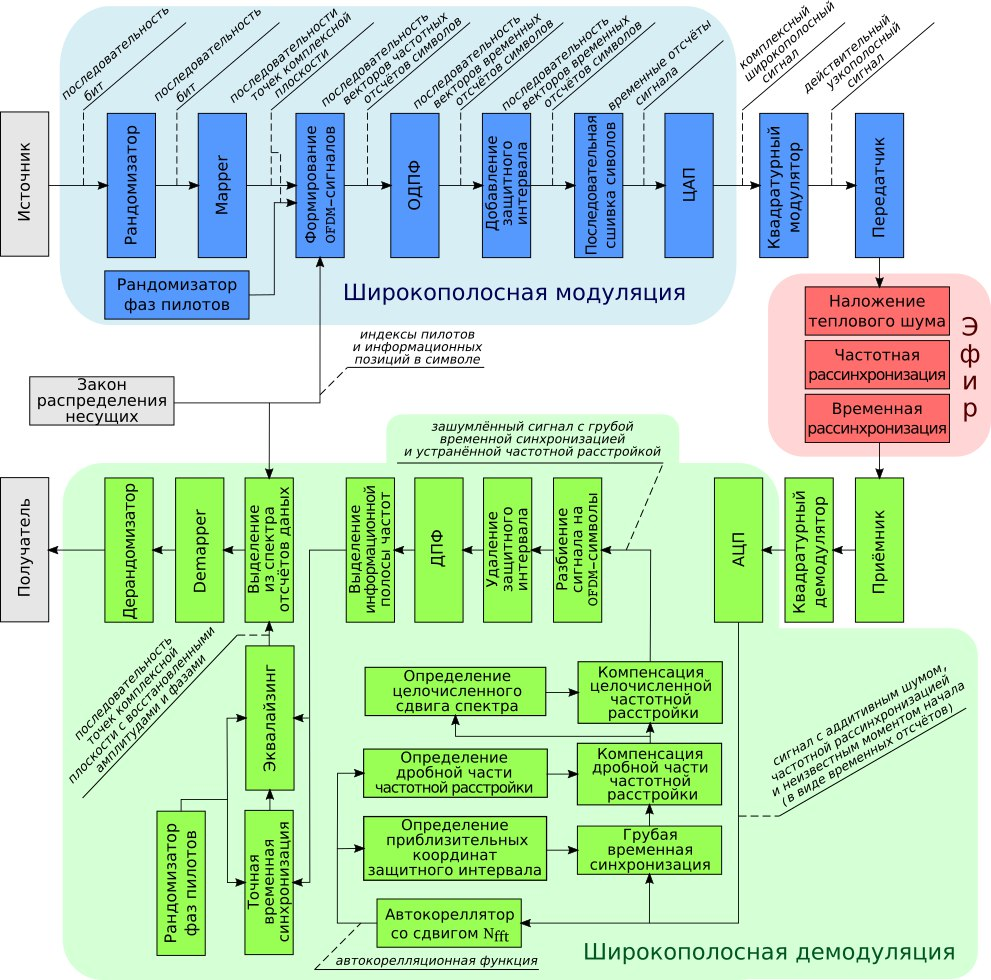
\includegraphics[width=1\textwidth]{schem11}
\caption{Схема обработки сигнала} \label{fg:schem0}
\end{figure}

\subsection{Первый этап. Простейший цикл передачи-приема}
Требуется сформировать простейший 'жизненный цикл' сигнала.
Считать, что канал идеальный и не вносит искажений.
Последовательность преобразований отображена на Рис.\ref{fg:schem1}) 
\begin{figure}[H]
\centering
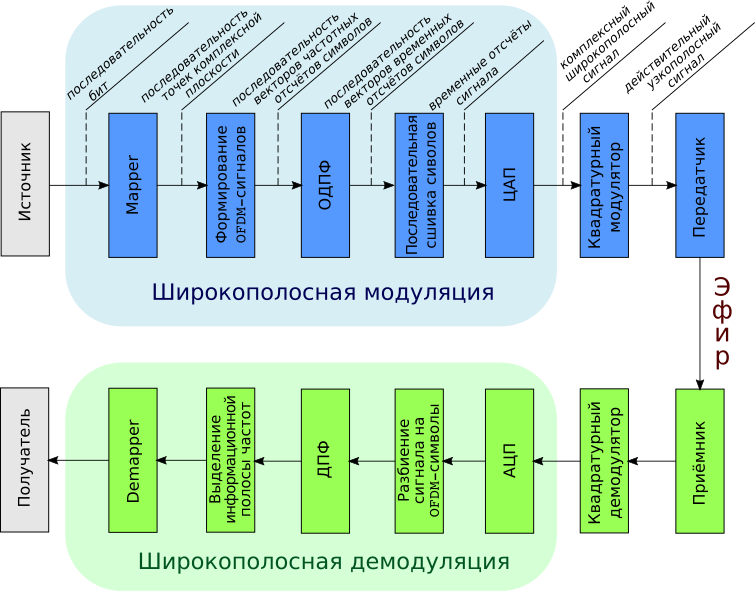
\includegraphics[width=1\textwidth]{OFDM-1}
\caption{Схема обработки сигнала} \label{fg:schem1}
\end{figure}

Рекомендуется осуществлять каждый этап преобразования в виде отдельной функции, что бы отслеживать результаты. 

Нам потребуются следующие входные параметры модели:
\begin{itemize}
\item \textit{n\underline{ }carriers} - число несущих сигнала (по дефолту 400).  (ссылка)
\item \textit{n\underline{ }fft} - порядок преобразования Фурье (1024 или 2048)  (ссылка)
\item \textit{constellation} - параметр, задающий модуляцию. В простейшем случае BPSK, либо QPSK, либо 16-QAM (ссылка)
\end{itemize}

Эти переменные считаются параметрами приемопередающей системы,  известными как на передатчике, так и на приемнике.

\subsubsection{Передатчик}
\subsubsection*{Формирование битовой последовательности}

Входную битовую последовательность можно сформировать случайным образом или импортировать из реального файла.
Второе сделать предпочтительнее, так как данные в изображениях сильно кореллированны. Это позволит пронаблюдать характерные особенности сигнала, например, периодичности,  соответствующие блокам изображения с одинаковыми цветами.  (вставить рисунок сигнала пик фактора для битов из картинки)

Результатом выполнения функции должна быть некоторая последовательность нулей и единиц:

$ 100101111110010000 ...$

\subsubsection*{Маппер}
Маппер - функция, которая осуществляет отображение групп битов на комплексную плоскость. 
В пункте (ссылка)
описаны различные варианты модуляций. 
Предлагается выбирать тип в зависимости от параметра \textit{constellation}.
Данный параметр определяет разрядность одного отсчета (например, для кодирования всех точек 16 QAM требуется 4 бита, для QPSK  - 2 бита и, соответственно, для BPSK - 1) (см. Рис.\ref{fg:constellations}).

\begin{figure}[h!]
\centering
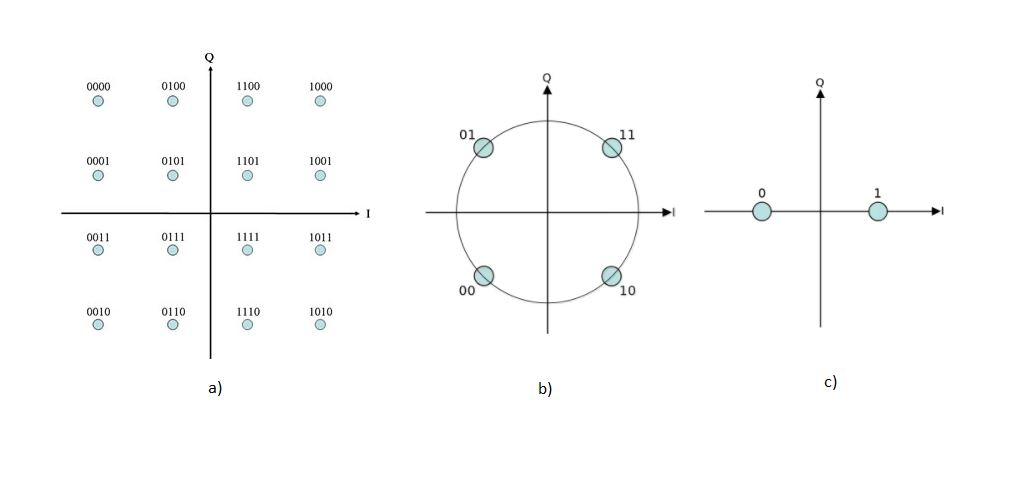
\includegraphics[width=1\textwidth]{constellations}
\caption{Типы созвездий: a)16-QAM;  b)QPSK;  c)BPSK} \label{fg:constellations}
\end{figure}

При составлении созвездия необходимо использовать коды Грея, что бы минимизировать ошибку при неверном распознавании.(ссылка)
Входной поток битов делится на 4ки или 2ки бит, которым в соответствие ставится точка из созвездия:

\begin{figure}[H]
\centering
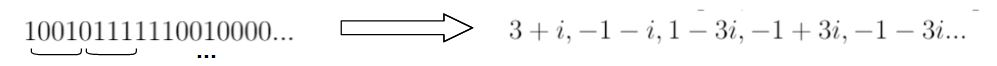
\includegraphics[width=1\textwidth]{schem2}
\end{figure}
 
 На выходе функции остается последовательность точек комплексной плоскости. 

\subsubsection*{Формирование OFDM-символа}

OFDM-модуляция предполагает частотное разделение сигнала. 
Передача информации в канале осуществляется пачками (они же OFDM-символы). 
В полосе выделяется  \textit{n\underline{ }carriers} поднесущих частоты, каждая из которых за время передачи одного символа несет информацию об одной информационной точке.
Следовательно, возможна передача не более  \textit{n\underline{ }carriers} точек за раз. 

На практике информационный объем одной передачи снижается, например, при выделении пилотных несущих (см последний этап), или при резервировании тона для снижения пик-фактора. 
Таким образом, целью данной функции является выделение необходимого числа точек из потока, а так же их подготовка к преобразованию Фурье. 
 
\subsubsection*{Преобразование Фурье}
 
Для передачи в настоящий физический канал сигнал требуется преобразовать в вид, доступный для передачи. 
А именно в аналоговую функцию, непрерывную по времени $S = S(t)$. 
По сути, совершить цифро-аналоговое преобразование. 

Поскольку мы моделируем цифровой сигнал, а не аналоговый 
воспользуемся теоремой Котельникова  (ссылка)
, которая позволяет рассматривать сигнал не как континуальный, а как набор дискретных отсчетов. 
Пока что наш сигнал представляет собой последовательность комплексных точек. 
Их можно считать частотными отсчетами, так как мы предполагаем, что каждая поднесущая несет информацию (фазу и амплитуду) об отдельной точке.  
Представить частотные отсчеты в виде функции от времени нам поможет преобразование Фурье.

Большинство современных языков программирования содержат готовые пакеты с преобразованием Фурье (алгоритм  Fast Fourier Transform и обратный ему), так что не будем изобретать велосипед и воспользуемся ими.
Тем более, что данный алгоритм достаточно сложен для понимания и потребует много времени. 

FFT принимает на вход последовательность дискретных временных отсчетов сигнала и возвращает дискретную последовательность отсчетов частотных. iFFT,  соответственно, производит обратную операцию. 
Поэтому на текущем этапе обработки сигнала нас интересует именно обратное преобразование, поскольку дальше сигнал отправится в канал
(см. Рис.\ref{fg:fft})


\begin{figure}[!h]
\centering
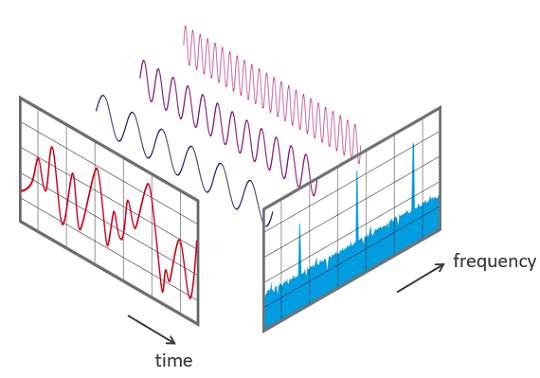
\includegraphics[]{FFT.png}
\caption{FFT} \label{fg:fft}
\end{figure}

Перед непоследственно самим преобразованием необходимо дополнить последовательность отсчетов нулями от значения \textit{n\underline{ }carriers} до \textit{n\underline{ }fft} (операция upsempling)
Делается это по нескольким причинам.
Прежде всего, исходят из особенностей алгоритма: преобразования на $2^n$ отсчетов проиходят существенно быстрее. 
Кроме того, upsempling позволяет существенно уплотнить временные отсчеты, так как имея всего \textit{n\underline{ }carriers} частотных отсчетов, мы получим целых \textit{n\underline{ }fft} временных. 
Сравните плотность отсчетов на Рис.\ref{fg:fft400} a) и b).

\begin{figure}[h!]
\begin{minipage}[h]{\linewidth}
\center{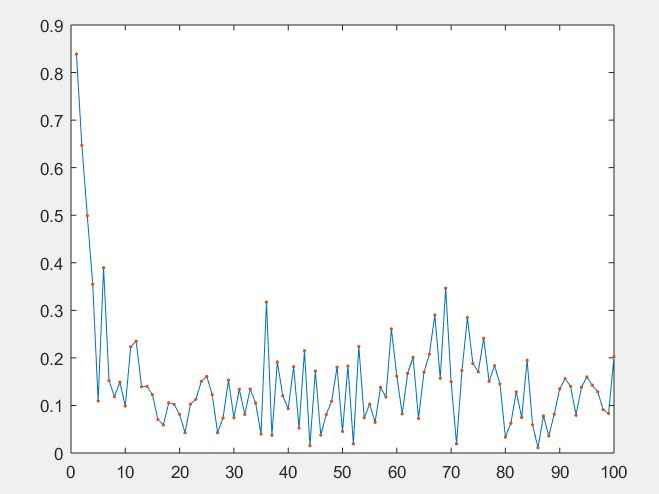
\includegraphics[width=0.5\linewidth]{fft400} \\ a)}
\end{minipage}
\begin{minipage}[h]{\linewidth}
\center{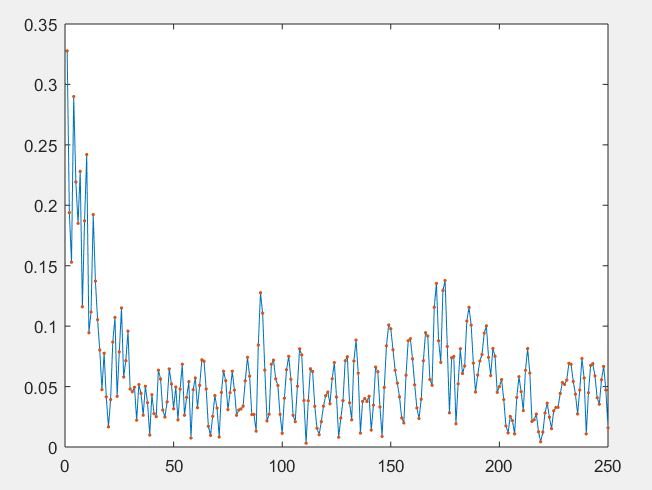
\includegraphics[width=0.5\linewidth]{fft1024} \\ b)}
\end{minipage}
\caption{Часть сигнала для a)400 отсчетов и b)1024 отсчетов.}
\label{fg:fft400}
\end{figure}

Выходом данного преобразования будет последовательность временных отсчетов сигнала.

 \subsubsection*{Передача символьной последовательности в канал}
 
Для каждого OFDM-символа формируется кусочек сигнала, которые необходимо "сшить" вместе перед передачей. 
Позднее здесь будет добавлен защитный интервал, сейчас можно просто склеить результаты iFFT-преобразования.

\subsubsection{Канал}

Канал считается идеальным, так что на этом этапе он не моделируется. 

\subsubsection{Приемник}

 \subsubsection*{Разбиение на символы на принимающей стороне}
 Все дальнейшие преобразования происходят на приемнике.
 Пока что не требуется проводить синхронизацию, так как канал идеален, и прием начинается с первого отсчета первого символа. 
 Аналогично как и в передатчике, следует разбить принятый сигнал на отдельные OFDM-символы для дальнейшего перобразования Фурье. 
 
\subsubsection*{Преобразование Фурье}
Необходимо выполнить аналого цифровое преобразование символа,  что бы получть значения отдельных частотных отсчетов.
Для этого применяем брпрямое преобразование Фурье (FFT).
На выходе получим набор точек комплексной плоскости.

\subsubsection*{Выделение информационной полосы частот}
Поскольку мы дополнили сигнал нулями, необходимо отбросить лишние частотные составляющие, которые не несут никакой информации. 
На  текущем этапе их можно просто отбросить.
на выходе должны получить  n\underline{ }carriers точек.  

\subsubsection*{Демаппер} 

Демаппер выполняет функцию обратную мапперу - отображение комплексных чисел в двоичный битовый вид.(ссылка) 
Однако напрямую отображать принятую точку нельзя - следует учесть ошибки (они появляются даже при идеальном канале, однако состаляют не более $O(10^-4)$, так как вызваны вычислительными ошибками алгаритма FFT). 
То есть демаппер должен вынести решение с учетом ошибки для каждой точки: какое значение передавалось изначально. 
Можно реализовать жесткое (зональное) или мягкое (вероятностное) решение. 

Жествкое принятие решений предполагает выделение областей принятия решения. При попадении точки в какую либо из областей выносится однозначное решение о ее значении. 
В простейшей реализации комплексная плоскость разбивается на участки. 
См Рис  \ref{fg:demap}
\begin{figure}[h!]
\centering
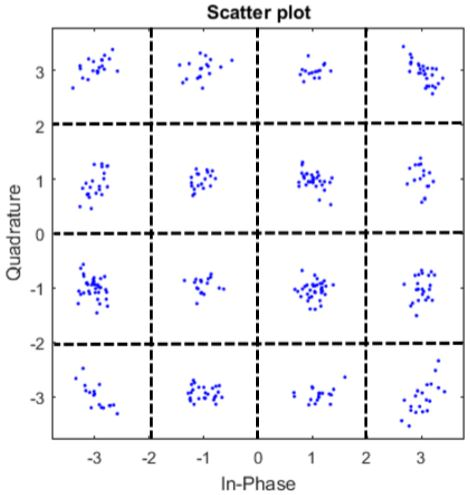
\includegraphics[]{demap}
\caption{Области принятия решения} \label{fg:demap}
\end{figure}

Однако такая реализация может быть очень громоздкой, особенно для числа точек более 4-х.
Поэтому удобнее разбивать на зоны не квадратами, а кругами. 
Для каждой точки высчитывается вектор ошибок - расстояний до точек созвездия. 
В качестве решения выбираетя точка созвездия с минимальной ошибкой.

Мягкое принятие решений основано на вычислении вероятностей. 
Может быть реализовано на основе вычисления MER (Modulation Error Ratio)

(??)

На выходе функции демаппера должен быть поток бит.

\subsubsection*{Контроль принятой информации} 

На этом обработка сигнала завершается. 
Что бы проверить эффективность модели необходимо убедиться, что принятый поток бит эквивалентен исходному. 
Для этого предлагается выполнить операцию XOR (исключающее или) над исходными битами и результатом работы демаппера.
Тогда, если последовательности совпадают, результатом функции будет нуль для каждого бита.
См. Рис.  \ref{fg:xor}

\begin{figure}[h!]
\centering
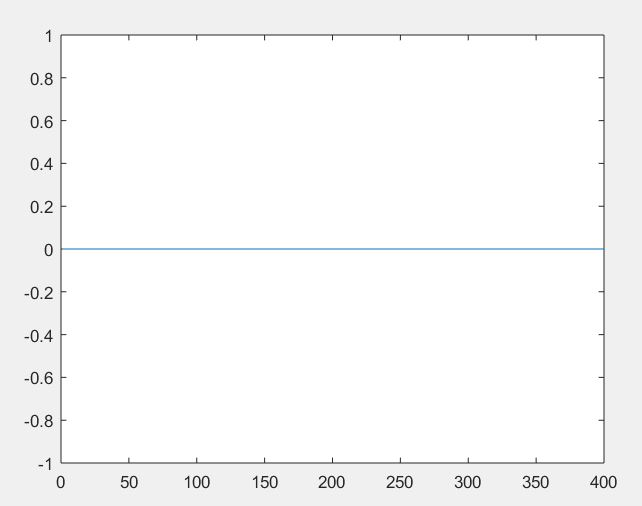
\includegraphics[]{xor}
\caption{XOR исходного и правильно обработанного потока бит} \label{fg:xor}
\end{figure}

\subsubsection{Вопросы и задания}
\begin{enumerate} %% Может, сделаем подпунктом второго уровня, чтобы номера подпунктов первого уровня совпадали с номером этапа?
\item 
Как влияет на сигнал изменение числа несущих или числа отсчетов в FFT?

\end{enumerate}














